\section{Multi-agent competition}
\label{sec:multi-agent}

In the multi-agent competition, the goal is to develop a DCOP algorithm in RMASBench. We choose to implement eXtreme-Ants \citep{Santos&Bazzan2009optmas}. This algorithm follows the extended generalized assignment problem (E-GAP) model of \citep{Scerri+2005} and extends Swarm-GAP \citep{Ferreira+2008ccmms}, a swarm intelligence-inspired task allocation algorithm for dynamic scenarios by explicitly employing a recruiting mechanism.

\subsection{Extended Generalized Assignment Problem (E-GAP)}
\label{sec:egap}
In E-GAP, a set of agents must be assigned to a set of tasks along discrete timesteps. Each agent has a given capability to perform each task. Capability can be regarded as the skill of the agent to perform the task. Each task consumes resources from the agent who performs it.


 %can be formalized as follows: let $\taskset$ be the set of tasks and $\agentset$ the set of agents. Each agent $i \in \agentset$ has $\agtres{i}$ resources to perform tasks. Each task $j \in \taskset$ consumes $\consumes{i}{j}$ resources of agent $i$, when it performs the task. Each agent $i$ has a capability $\agtcap{i}{j} \in [0,1]$ to perform task $j$. Capability can be regarded as the skill of the agent to perform the task. %A value of $\agtcap{i}{j}$ close to $1$ means that $i$ performs $j$ with high speed or quality.

%An allocation matrix $A_{|\agentset| \times |\taskset|}$ has an element $\allocate{i}{j}$ set to $1$ if agent $i$ performs task $j$, and 0 otherwise. 
An agent may perform multiple tasks but a task cannot be performed by more than one agent. Thus, a task that would require multiple agents to execute it must be broken down into smaller, inter-related tasks. %In the case that all inter-related tasks must be simultaneously allocated, they are AND-constrained, i.e., they are related by an AND constraint. 

%Formally, let  $\allandtasks \enspace = \{\andtasks{1},\cdots,\andtasks{p} \}$, where $\andtasks{k} = \{j_{k_1},\cdots,j_{k_q}\}$ denotes the $k$-th set of AND-constrained tasks. 

%$\partialrwd{i}{j}$

The partial reward given by the allocation of a task by an agent depends on the agent capability to perform the task and whether the task is inter-related with others. 

%The first case refers to an unconstrained task, the second case refers to an AND-constrained task that belongs to a set where all other constrained tasks were allocated and the third case refers to an AND-constrained task that belongs to a set where one or more constrained task was not allocated.

%Eq. \ref{eq:egap-partial-reward}

%\begin{equation}
%\label{eq:egap-partial-reward}
%\partialrwd{i}{j} = 
%\begin{cases}
%  \agtcap{i}{j} \times \allocate{i}{j} ,& \text{if } \forall\andtasks{k} \in \enspace \allandtasks, j \notin \andtasks{k}\\
%  \agtcap{i}{j} \times \allocate{i}{j} ,& \text{if } \exists\andtasks{k} \in \enspace \allandtasks \text{ with } j \in \andtasks{k} \wedge \sum_{i \in \agentset}\sum_{j_k \in \andtasks{k}} \allocate{i}{j_k} = |\andtasks{k}| %\forall j_{k_u} \in \alpha_k, a_{xj_{k_u}} \neq 0 
%  \\
%  0,& \text{otherwise}
%\end{cases}
%\end{equation}


In E-GAP, the total reward is calculated as the sum of the partial rewards of the agents along discrete timesteps. A delay cost is applied as a penalty for not allocating a task in a given timestep. The constraints are that the agents must allocate tasks within their resource limits and that a task can be performed by at most one agent.

%Thus, all variables are indexed by the timestep $t$. In a given timestep, the reward is the sum of partial rewards calculated via Eq. \ref{eq:egap-partial-reward}. 
 %The calculation of rewards along the timesteps captures the dynamics of the environment. That is, the reward in a given timestep depends on the tasks and agents that exist in that timestep. 
%Equation \ref{eq:egap-total-reward2} determines that agents must allocate tasks within their resource limits and Eq. \ref{eq:egap-total-reward3} determines that a task can be performed by only one agent. %Thus, large tasks must be broken down into smaller tasks that can be performed by a single agent. E-GAP also considers task interdependence, but this aspect will not be investigated in this work. 
%The goal in E-GAP is to maximize the total reward $W$ given by Eq. \ref{eq:egap-total-reward}. Note that terms which are indexed by the timestep $t$ might vary from one timestep to another. For example, new tasks can arise, the resources of the agents might be reduced, etc.
%A Eq. \ref{eq:egap-total-reward} possui semelhança com a Eq. \ref{eq:gap-optimal}, 

%\begin{subequations}
%	\begin{equation}
%	\label{eq:egap-total-reward1}
%	W = \sum_t \sum_{i^t \in \agentset^t} \sum_{j^t \in \taskset^t} w_{ij}^t \times a_{ij}^t - 
%	\sum_t \sum_{j^t \in \taskset^t}(1 - a_{ij}^t) \times d_j^t 
%	\end{equation}
%	
%	\begin{equation}
%	\label{eq:egap-total-reward2}
%	\text{ subject to:~~~~~~~~}	
%	\forall t \forall i^t \in \agentset^t, \sum_{j^t \in \taskset^t} \consumes{i}{j}^t \times a_{ij}^t \leq \agtres{i}^t 
%	\end{equation}
%	\begin{equation}
%	\label{eq:egap-total-reward3}
%	\text{and:~~~~~~~~~}
%	\forall t \forall j^t \in \taskset^t, \sum_{i^t \in \agentset^t} a_{ij}^t \leq 1 
%	\end{equation}
%\end{subequations}
\subsection{Description of eXtreme-Ants}
\label{sec:x-ants}
Inspired by the division of labor in social insects, eXtreme-Ants is an approximate algorithm for the E-GAP. %In swarms, or colonies of social insects, complex behaviors emerge from the aggregation of individual actions of colony members. %One characteristic of swarms is the ability to respond to changes in the environment by adjusting the numbers of members performing each task.

Observations about swarm behaviors are the base of the model presented in \citep{Theraulaz+1998}, where tasks have associated stimulus %\footnote{Stimulus intensity may be associated with pheromone concentration, the number of encounters with other individuals performing the task or another characteristic that individuals can measure.} 
and individuals have response thresholds for each task. Let $\stimulus{j} \in [0,1]$ be the stimulus associated with task $j$ and $\respthresh{i}{j} \in [0,1]$ be the response threshold of individual (agent) $i$ to task $j$. The tendency, or probability, of individual $i$ to engage in task $j$ is denoted by $\tendency{i}{j} \in [0,1]$. The response threshold \respthresh{i}{j} of individual $i$ to task $j$ depends on $i$'s capability to perform $j$ ($\agtcap{i}{j} \in [0,1]$). The calculation of \respthresh{i}{j} and \tendency{i}{j} is shown in Eq. \ref{eq:tendency}.

\begin{equation}
\label{eq:tendency}
\tendency{i}{j} = \frac{\stimulus{j}^2}{\stimulus{j}^2 + \respthresh{i}{j}^2} 
\qquad\text{and}\qquad
\respthresh{i}{j} = 1 - \agtcap{i}{j} 
\end{equation}

%In swarms, due to polymorphism, individuals may be more able to perform certain kinds of tasks. 
%The response threshold \respthresh{i}{j} of individual $i$ to task $j$ is calculated via Eq. \ref{eq:respthresh}, where $\agtcap{i}{j} \in [0,1]$ is the capability of agent $i$ to perform task $j$.
%
%\begin{equation}
%\label{eq:respthresh}
%\respthresh{i}{j} = 1 - \agtcap{i}{j} 
%\end{equation}

Regarding independent, i.e., tasks that are not inter-related, in eXtreme-Ants, agents individually decide which task they will engage in a simple and efficient way (via Eq. \ref{eq:tendency}), minimizing computational effort and communication between agents. Agents communicate using a token mechanism. When a given agent perceives new tasks, it creates a token with these tasks. The agent can receive tokens from other agents too. Either way, the holder of a token has the right to decide in which tasks of the token it will engage. The token with the remaining tasks is passed to a random agent that has not held the token before. %This is formalized in Alg. \ref{alg:x-ants}, which is executed by each agent independently.

%\begin{algorithm}[ht]
%\begin{algorithmic}
%\STATE When tasks are perceived: $token \gets$ \{perceived tasks\}
%\STATE When message is received: $token \gets$ \{received token\}
%
%\FORALL{task $j \in token$} 
%\STATE{Compute and normalize \tendency{i}{j} for all tasks in $token$}
%\IF{$random() < \tendency{i}{j}$ and $\agtres{i} > c_{ij}$ }
%\STATE{Engage in task $j$}
%\STATE{$token \gets token \setminus \{j\}$}
%\STATE{$\agtres{i} \gets \agtres{i} - c_{ij}$}
%\ENDIF
%\ENDFOR
%
%\STATE Send $token$ to random agent that didn't see the token before
%\end{algorithmic}
%\caption{Non-constrained task monitor}
%\label{alg:x-ants}
%\end{algorithm}

To deal with inter-related tasks, i.e. groups of tasks that demand simultaneous execution, eXtreme-Ants uses a process inspired in the recruitment process for cooperative transport observed among ants. When an agent perceives a set of inter-related tasks, it acts as a scout ant. Firstly it attempts to allocate all the constrained tasks. If it fails, then it begins a recruitment process via communication. There are five kinds of messages used in the recruitment protocol of eXtreme-Ants: \msg{request}, \msg{committed}, \msg{engage}, \msg{release} and \msg{timeout}. Figure \ref{fig:auction} illustrates the recruitment process, except the timeout mechanism. %An agent decides to commit to a task probabilistically, via Eq. \ref{eq:tendency}. 

\begin{figure}[ht]
  \centering
  \subfigure[]{
    {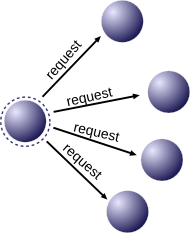
\includegraphics[width=2.4cm]{img/request.png}}
    \label{fig:request}
  }%
  \subfigure[]{
    {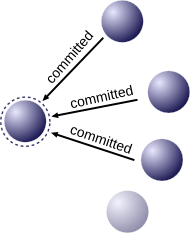
\includegraphics[width=2.4cm]{img/offer.png}}
    \label{fig:offer}
  }%
  \subfigure[]{
    {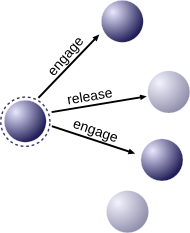
\includegraphics[width=2.4cm]{img/commit.png}}
    \label{fig:commit}
  }%

  \caption{Recruitment process: \subref{fig:request} recruiter (circled with dashed line) sends \msg{request} messages; \subref{fig:offer} agents who decide to help respond with \msg{committed} messages; \subref{fig:commit} recruiter sends \msg{engage} to selected teammates and dismisses non-selected ones with \msg{release} messages.}

 \label{fig:auction}
\end{figure}

In addition to the steps presented in Fig. \ref{fig:auction}, in eXtreme-Ants, a \msg{request} message is forwarded when the agent who received it decides to not commit to the task. Besides, there is a mechanism to prevent excessive forwarding of \msg{request} messages: when a \msg{request} message is forwarded too many times, it expires. The agent that received an expired \msg{request} message sends a \msg{timeout} message to the scout (recruiter) agent. The scout, upon receipt of \msg{timeout} messages, sends \msg{release} messages to dismiss agents that had previously committed to the task. 

%The choice of eXtreme-Ants for the multi-agent competition is due to its performance in terms of team reward, computational effort and exchanged messages compared to other E-GAP-based algorithms. Also, it would be interesting to compare its performance with factor-graph based algorithms, such as max-sum, which is implemented in RMASBench \citep{Kleiner+2013}. 

This TDP presents a brief description of eXtreme-Ants. For further details, the reader can refer to \citep{Santos&Bazzan2009optmas}.

%The recruitment process used in the Agent competition (Section \ref{sec:recruiting}) a simplification of the recruitment process of eXtreme-Ants. %Thus, Fig. \ref{fig:auction} also illustrates the recruitment process presented here. 
%In the agent competition we use a simplified version of
%A \textit{timeout} message informs that a request for a task has reached its timeout, and is used to prevent deadlocks. The handling of AND-constrained tasks is formalized in Alg. \ref{alg:x-ants-comm}.

%
%\begin{algorithm}[ht]
%\begin{algorithmic}
%\STATE When set of constrained tasks \andtasks{} is perceived:
%\STATE{$\beta \gets \emptyset$}
%\IF{ $\agtres{i} \geq \sum_{j \in \andtasks{}} \consumes{i}{j}$}
%	\STATE{Compute and normalize \tendency{i}{j} for all tasks in token}
%	\FORALL{task $j \in \andtasks{}$}
%		\IF{$random() < \tendency{i}{j}$ }
%			\STATE{Accept task $j$; $\beta \gets \beta \cup \{j\}$; $\andtasks{} \gets \andtasks{} \setminus \{j\}$}
%		\ENDIF
%		\IF{All tasks in $\andtasks{}$ were accepted, i.e., $\beta = \andtasks{}$}
%			\STATE{Perform all tasks and set $\agtres{i} \gets \agtres{i} - \sum_{j \in \andtasks{}} \consumes{i}{j}$}
%		%\ELSE
%		%	\STATE{Discard all accepted tasks and set: $\andtasks{} \gets \andtasks{} \cup \beta$}
%	    \ENDIF
%    \ENDFOR 
%\ENDIF
%\STATE{recruit($\andtasks{} \setminus \beta$)}
%\end{algorithmic}
%\caption{Constrained task monitor}
%\label{alg:x-ants-comm}
%\end{algorithm}


%\subsection{E-GAP as a DCOP}
%
%In a DCOP, each agent has a variable to which it must assign values corresponding to the tasks it will perform. In the E-GAP, agents may execute multiple tasks at once, thus, DCOP variables may take multiple values simultaneously, as in graph multi-coloring \citep{Scerri+2005}. However, a task cannot be performed by more than one agent. Thus, the same value cannot be assigned to two distinct DCOP variables. This implies a "not-equal" constraint between every agent that can perform the same tasks, which results in dense constraint graphs, which are problematic in DCOP because of the large ammount of commnication required to remove conflicts \citep{Scerri+2005}.
%
%E-GAP-based task allocation algorithms (e.g. LA-DCOP \citep{Scerri+2005}, Swarm-GAP \citep{Ferreira+2008ccmms}, eXtreme Ants \citep{Santos&Bazzan2009optmas}}) use a token mechanism to avoid the communication issue. Tasks are grouped in tokens that are owned by a single agent. Only the token owner may allocate the tasks in it. The token owner may forward it to a teammate. This avoids conflicts and reduces communication.

%A DCOP is a tuple (\variables, \domains, \functions). $\variables = \{x_1,\cdots,x_{|\variables|}\}$ is the set of variables, $\domains = \{D_1,\cdots D_{|\variables|}\}$ is the set of finite and discrete domains, such that each $x_i \in \variables$ takes values in $D_i \in \domains$. Each agent owns a variable and decides which value it will take. \functions~ is the set of functions that define costs of variable assignments. In a DCOP, the goal is to minimize the sum of the costs of functions in \functions. 

%The E-GAP can be formulated as a DCOP as follows:
%
%\begin{itemize}
%%  \item Cada variável $x_i \in V$ representa um agente $i \in \agentset$.
%  \item Let $2^\domains$ be the power set of $\taskset$. Domain $D_i$ of variable $x_i$ is the set of elements in $2^\domains$ such that $\forall d \in D_i, \sum_{j \in d} \rescspt{i}{j} \leq \agtres{i}$. This means that $D_i$ is a set composed of sets of tasks that agent $i$ can perform simultaneously.
%  \item A cost function $f_{kl}$, related to variables $x_k$ e $x_l$ is given by Eq. \ref{eq:dcop-constraint-cost}. The cost (to be minimzed) is the dual of the sum of rewards (to be maximized in E-GAP) obtained by agents $k$ and $l$ via Eq. \ref{eq:egap-partial-reward}. Besides, the function prevents that the same task is allocated by two agents.
%
%\begin{equation}
%\label{eq:dcop-constraint-cost}
%f_{kl} = 
%\begin{cases}
%  - \left(\sum_{j \in D_k} w_{kj} + \sum_{j \in D_l} w_{lj}\right) ,& \text{se } a_{kj} \neq a_{lj}\\
%  \infty,& \text{caso contrário}
%\end{cases}
%\end{equation}
%
%%Uma restrição com o custo dado pela Equação \ref{eq:dcop-constraint-cost} é criada para cada par de variáveis em $V$. 
%\end{itemize}
%The constraint graph of this DCOP formulation is complete, as there is a constraint between each pair of variables. The total number of constraints can be calculated as $\frac{|\variables|(|\variables|-1)}{2}$. The number of constraints grows quadratically with the number of agents (as each agent is represented by a variable). The domain of the variables, on the worst case, where all agents can allocate all tasks is $2^{t}$ where $t$ is the number of tasks. That is, the domain grows exponentially with the number of tasks. This complex DCOP model requires approximate algorithms to be solved.
%
%

